\subsection*{a}
List of all intermediate clusters and their centers:
\begin{verbatim}
Iteration 0:
cluster 1: center=[2.000, 12.000]; points=[A ]
cluster 2: center=[3.000, 11.000]; points=[B ]
cluster 3: center=[3.000, 8.000]; points=[C D E F G H ]

Iteration 1:
cluster 1: center=[2.000, 12.000]; points=[A ]
cluster 2: center=[3.000, 11.000]; points=[B C ]
cluster 3: center=[7.500, 6.000]; points=[D E F G H ]

Iteration 2:
cluster 1: center=[2.000, 12.000]; points=[A B ]
cluster 2: center=[3.000, 9.500]; points=[C ]
cluster 3: center=[8.400, 5.600]; points=[D E F G H ]

Iteration 3:
cluster 1: center=[2.500, 11.500]; points=[A B ]
cluster 2: center=[3.000, 8.000]; points=[C ]
cluster 3: center=[8.400, 5.600]; points=[D E F G H ]
\end{verbatim}
\newpage
\subsection*{b}
\begin{figure}[h!]
	\centering
	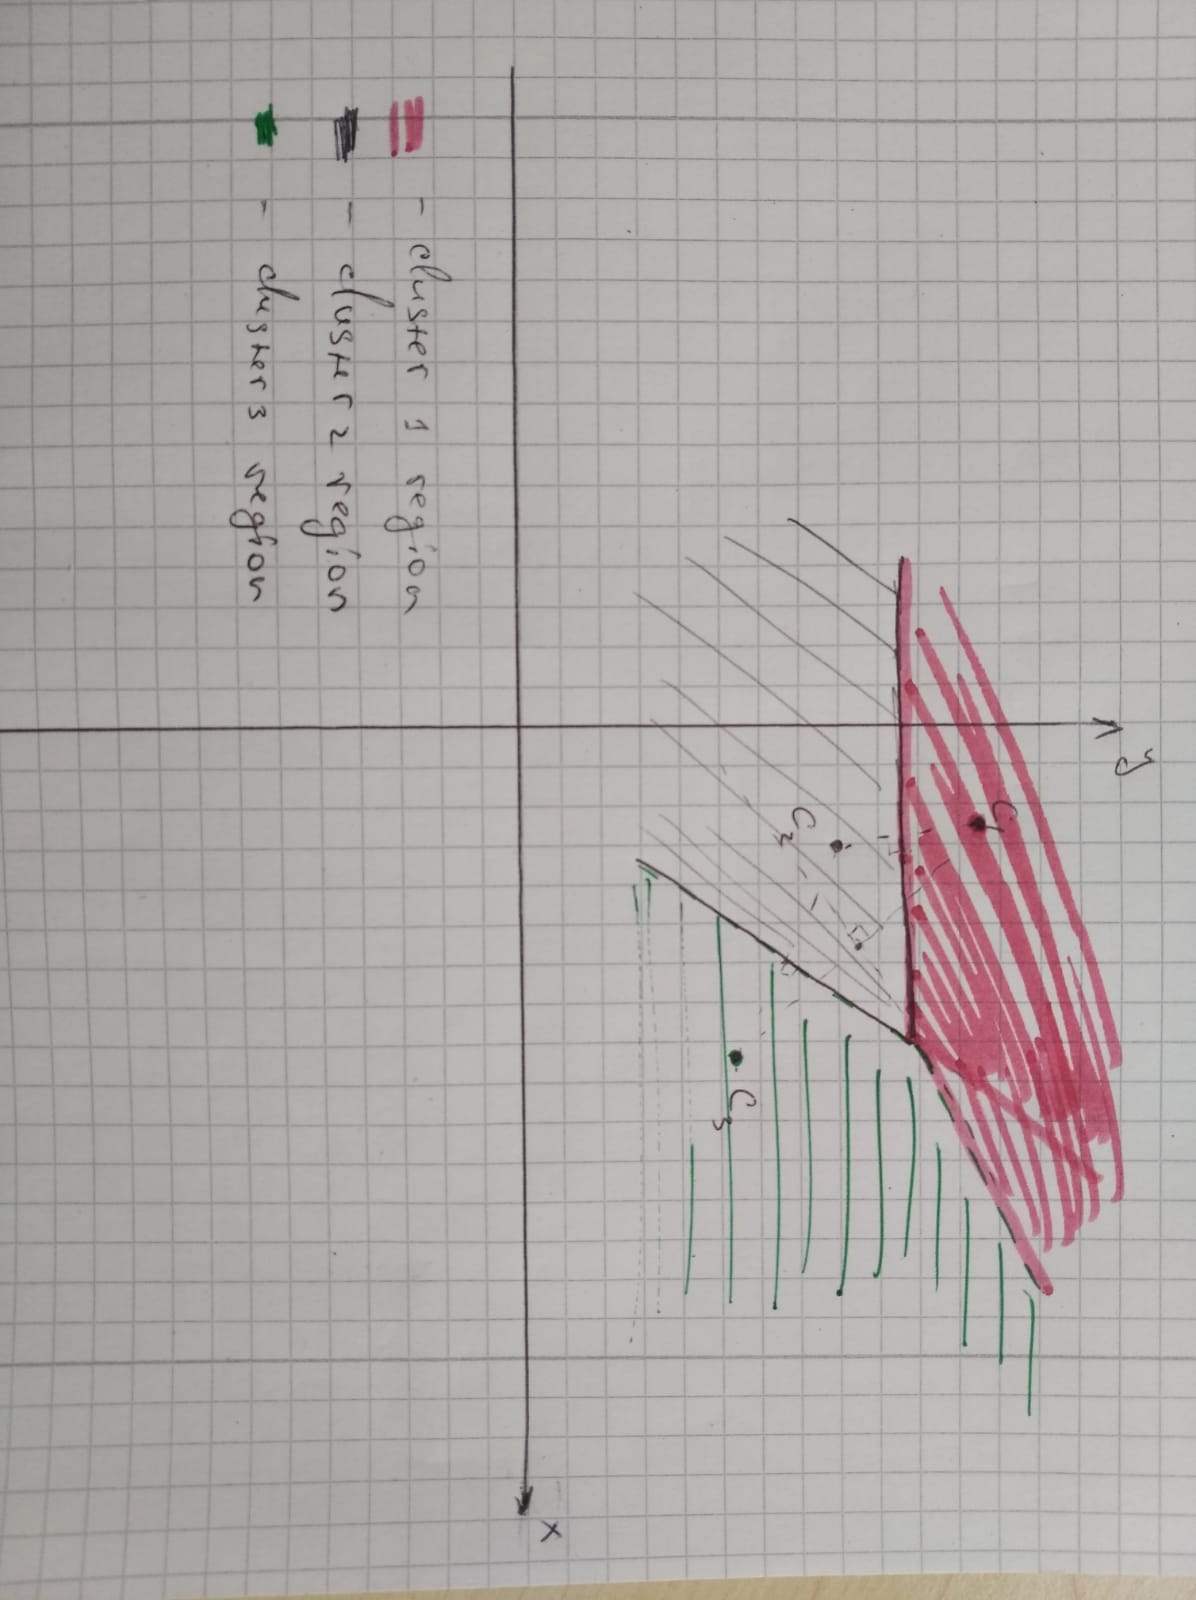
\includegraphics[width=\linewidth, angle=90]{task4b.jpeg}
	\caption{Cluster centers and their respective areas}
\end{figure}
Given points $A$ and $B$, and hyperplane $L$, which is perpendicular to segment $AB$ and intersects $AB$ in the middle
and points A and N lie on the same side of the hyperplane L prove, that $\forall points N on the same side with A w.r.t. hiperplane L: ||A-N|| < ||B-N||$.

Suppose we have projection N on AB: $\hat{N} = (N * \dfrac{(B-A)}{||B-A||}) \cdot \dfrac{B-A}{||B-A||}$.
$||A\hat{N}|| < ||B\hat{N}||$ while projection is parallel to hyperplane L and N and A are above the hyperplane by definition.
Thus by the n-dimensional Pythagorean theorem: 
\begin{enumerate}
	\item $||AN||^2 = ||A\hat{N}||^2 + ||N\hat{N}||^2$. 
	\item $||BN||^2 = ||B\hat{N}||^2 + ||N\hat{N}||^2$.
\end{enumerate} 
Then $||AN||^2 = ||A\hat{N}||^2 + ||BN||^2 -||B\hat{N}||^2$.
$||AN||^2 - ||BN||^2 = ||A\hat{N}||^2  - ||B\hat{N}||^2 < 0$, thus $||AN|||^2 < ||BN||^2$ and $||AN|| < ||BN||$.

\subsection{c}
Given points E,F,G as an initial cluster means the calculation gives the next results
\begin{verbatim}
Iteration 0:
cluster 1: center=[7.000, 5.000]; points=[A B C D E ]
cluster 2: center=[7.000, 3.000]; points=[F ]
cluster 3: center=[10.000, 8.000]; points=[G H ]

Iteration 1:
cluster 1: center=[4.000, 8.000]; points=[A B C ]
cluster 2: center=[7.000, 3.000]; points=[D E F ]
cluster 3: center=[11.500, 8.000]; points=[G H ]

Iteration 2:
cluster 1: center=[2.667, 10.333]; points=[A B C ]
cluster 2: center=[6.333, 4.000]; points=[D E F ]
cluster 3: center=[11.500, 8.000]; points=[G H ]
\end{verbatim}
\subsection{d}